%\pdfoutput=1
\documentclass[12pt,a4paper,reqno]{amsart}
\newcommand\hmmax{0}
\newcommand\bmmax{0}
\usepackage{amssymb}
\usepackage{amscd}
\usepackage[pdftex,pdfpagelabels]{hyperref}
\usepackage{enumerate}
\usepackage{comment}
%\usepackage{psfig}
\usepackage{graphicx}
\usepackage{cleveref}
\usepackage{siunitx}
\usepackage{tikz-cd}
\usepackage{stix}
\usepackage{bm}
\DeclareMathAlphabet\mathbfcal{LS2}{stixcal}{b}{n}
\numberwithin{equation}{section}

%\usepackage{mathabx}


\usepackage{mathtools}%                  http://www.ctan.org/pkg/mathtools
\usepackage[tableposition=top]{caption}% http://www.ctan.org/pkg/caption
\usepackage{booktabs,dcolumn}%           http://www.ctan.org/pkg/dcolumn + http://www.ctan.org/pkg/booktabs

% Lighter notation.
%\newcommand*\mc[1]{\multicolumn{1}{c}{#1}}
%\newcommand*\tupref[2]{\href{http://math.mit.edu/~primegaps/tuples/admissible_#1_#2.txt}{\num{#2}}}



%\DeclareMathOperator*\Kl{Kl} (commented because yield bad display for  \Kl_q %replaced with \newcommand... )
%\DeclareMathOperator*\FT{FT} (commented because yield bad display for \FT_q
%replaced with \newcommand...)

\DeclareMathOperator*\swan{swan}
\DeclareMathOperator*\cond{cond}
\DeclareMathOperator*\Gal{Gal}

\newcommand{\FT}{\mathrm{FT}}
\newcommand{\Kl}{\mathcal{K}\ell}
% Setup for ``caption''.
%\DeclareCaptionLabelSeparator{separation}{:\quad}
%\captionsetup{
  %font=small,
  %labelfont=sc,
  %labelsep=separation,
  %width=0.8\textwidth
%}

\DeclareFontFamily{OT1}{rsfs}{}
\DeclareFontShape{OT1}{rsfs}{n}{it}{<-> rsfs10}{}
\DeclareMathAlphabet{\mathscr}{OT1}{rsfs}{n}{it}

\addtolength{\textwidth}{3 truecm}
\addtolength{\textheight}{1 truecm}
\setlength{\voffset}{-.6 truecm}
\setlength{\hoffset}{-1.3 truecm}

\theoremstyle{plain}

\newtheorem{theorem}{Theorem}[section]
%\newtheorem{theorem}[theorem]{Theorem}
\newtheorem{proposition}[theorem]{Proposition}
\newtheorem{lemma}[theorem]{Lemma}
\newtheorem{corollary}[theorem]{Corollary}
\newtheorem{conjecture}[theorem]{Conjecture}
\newtheorem{heuristic}[theorem]{Heuristic}
\newtheorem{principle}[theorem]{Principle}
\newtheorem{question}[theorem]{Question}
\newtheorem{problem}[theorem]{Problem}
\newtheorem{claim}[theorem]{Claim}

\theoremstyle{definition}

%\newtheorem{roughdef}[subsection]{Rough Definition}
\newtheorem{definition}[theorem]{Definition}
\newtheorem{remark}[theorem]{Remark}
\newtheorem{remarks}[theorem]{Remarks}
\newtheorem{example}[theorem]{Example}
\newtheorem{examples}[theorem]{Examples}
%\newtheorem{problem}[subsection]{Problem}
%\newtheorem{question}[subsection]{Question}

\renewcommand\P{\mathbb{P}}
\newcommand\E{\mathbb{E}}
\newcommand\Var{\mathrm{Var}}
\newcommand\R{\mathbb{R}}
\newcommand\Z{\mathbb{Z}}
\newcommand\F{\mathbf{F}}
\newcommand\N{\mathbb{N}}
\newcommand\n{\mathbf{n}}
\renewcommand\a{\mathbf{a}}
\renewcommand\b{\mathbf{b}}
\renewcommand\j{\mathbf{j}}
\renewcommand\k{\mathbf{k}}
\renewcommand\v{\mathbf{v}}
\renewcommand\t{\mathbf{t}}
\renewcommand\r{\mathbf{r}}
\renewcommand\l{\mathbf{l}}
\newcommand\X{\mathbf{X}}
\newcommand\T{\mathbf{T}}
\newcommand\Y{\mathbf{Y}}
\newcommand\A{\mathbf{A}}
\newcommand\W{\mathbf{W}}
\newcommand\C{\mathbb{C}}
\newcommand\Q{\mathbb{Q}}
\renewcommand\Re{{\operatorname{Re}}}
\renewcommand\Im{{\operatorname{Im}}}
\newcommand\Log{{\operatorname{Log}}}
\newcommand\lcm{{\operatorname{lcm}}}
\renewcommand\gcd{{\operatorname{gcd}}}
\newcommand\eps{\varepsilon}
\newcommand\deriv{\zeta}
\newcommand\zero{\lambda}

\renewcommand{\mod}{\bmod}

\parindent 0mm
\parskip   5mm


\begin{document}

\title{Decomposing a factorial into large factors}

\author{Terence Tao}
\address{UCLA Department of Mathematics, Los Angeles, CA 90095-1555.}
\email{tao@math.ucla.edu}

%\email{}

\subjclass[2020]{11A51}

\begin{abstract}  Let $t(N)$ denote the largest number such that $N!$ can be expressed as the product of $N$ numbers greater than or equal to $t(N)$.
The bound $t(N)/N = 1/e-o(1)$ was apparently established in unpublished work of Erd\H{o}s, Selfridge, and Straus; but the proof is lost.  Here we obtain the more precise asymptotic bounds
$$ \frac{1}{e} - \frac{O(1)}{\log N} \leq \frac{t(N)}{N} \leq \frac{1}{e} - \frac{c_0+o(1)}{\log N}$$
for an explicit constant $c_0 \approx 0.3044$, answering a question of Erd\H{o}s and Graham.  Our methods are elementary, aside from the use of the prime number theorem (with classical error term).  Using an effective version of the upper bound argument, we also show that $t(N)/N < 1/e$ for $N \neq 1,2,4$, answering a question of Guy and Selfridge.
\end{abstract}

\maketitle

%%%%%%%%%%%%%%%%%%%%%%%%%%%%%%%%%%%%%%%%%%%%%%%%%

\section{Introduction}

For any natural number $N$, let $t(N)$ be the largest quantity such that one can express the factorial $N!$ as a product
\begin{equation}\label{an}
 N! = a_1 \dots a_N
\end{equation}
of $N$ factors $a_1,\dots,a_N \in \N$ that are each greater than or equal to $t(N)$. The first few elements of this sequence are
$$ 1,1,1,2,2,2,2,2,3,3,3,3,3,4, \dots$$
and the values of $t(N)$ for $N \leq 79$ may be found at \href{https://oeis.org/A034258}{OEIS A034258}. 


From the obvious lower bound
\begin{equation}\label{obvious}
  a_1 \dots a_N  \geq t(N)^N
\end{equation}
and Stirling's formula \eqref{stirling} we obtain the trivial upper bound
$$ \frac{t(N)}{N} \leq \frac{(N!)^{1/N}}{N} = \frac{1}{e} + O\left( \frac{\log N}{N}\right)$$
for $N \geq 2$; see \Cref{fig1}.  In \cite[p.75]{erdos-graham} it was reported that an unpublished work of Erd\H{o}s, Selfridge, and Straus established the asymptotic
\begin{equation}\label{t1}
  \frac{t(N)}{N} = \frac{1}{e} + o(1)
\end{equation}
(first conjectured in \cite{erdos-71}) and asked if one could show the bound
\begin{equation}\label{Tbound}
   \frac{t(N)}{N} \leq \frac{1}{e} - \frac{c}{\log N}
\end{equation}
for some constant $c>0$ (problem {\#}391 in \url{https://www.erdosproblems.com}; see also \cite[Section B22, p. 122--123]{guy}); it was also noted that similar results were obtained in \cite{algr77} if one restricted the $a_i$ to be prime powers.  However, as later reported in \cite{erdos-96}, Erd\H{o}s ``believed that Straus had written up our proof [of \eqref{t1}]. Unfortunately Straus suddenly died and no trace was ever found of his notes. Furthermore, we never could reconstruct our proof, so our assertion now can be called only a conjecture''.   In \cite{guy} the lower bound $\frac{t(N)}{N} \geq \frac{1}{4}$ was established for sufficiently large $N$, by rearranging powers of $2$ and $3$ in the obvious factorization $1 \times 2 \times \dots \times N$ of $N!$.  A variant lower bound of the asymptotic shape $\frac{t(N)}{N} \geq \frac{3}{16}-o(1)$ obtained by rearranging only powers of $2$, and which is superior for medium values of $N$, can also be found in \cite{guy}.

In this note we recover and strengthen these results, and in particular obtain a positive answer to the question in \cite{erdos-graham}.

\begin{theorem}\label{main} For sufficiently large $N$, one has
  $$ \frac{1}{e} - \frac{O(1)}{\log N} \leq \frac{t(N)}{N} \leq \frac{1}{e} - \frac{c_0+o(1)}{\log N}$$
where
  \begin{align*}
    c_0 &\coloneqq \frac{1}{e} \int_0^1 \left \lfloor \frac{1}{x} \right\rfloor \log \left( ex \left \lceil \frac{1}{ex} \right\rceil \right)\ dx \\
    &= \frac{1}{e} \int_1^\infty \lfloor y \rfloor \log \frac{\lceil y/e \rceil}{y/e}\ \frac{dy}{y^2} \\
    &= 0.3044\dots
  \end{align*}
(see \Cref{fig-mean}).  In particular, \eqref{t1} and \eqref{Tbound} hold.
\end{theorem}

\begin{figure}
  \centering
  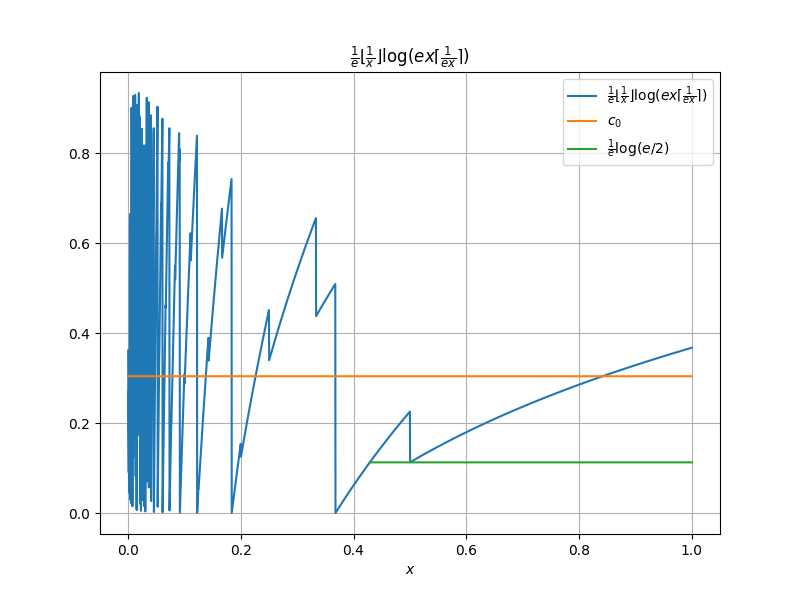
\includegraphics[width=0.8\textwidth]{integ.png}
  \caption{The piecewise continuous function $x\mapsto \frac{1}{e} \left \lfloor \frac{1}{x} \right\rfloor \log( ex \left \lceil \frac{1}{ex} \right\rceil)$, together with its mean value $c_0 = 0.3044\dots$.  The function exhibits an oscillatory singularity at $x=0$ similar to $\sin \frac{1}{x}$ (but it is always nonnegative and bounded). We also display the (crude) lower bound of $\frac{1}{e} \log(e/2)$ for $x \geq \frac{1}{\sqrt{2e}} = 0.4288\dots$. Informally, this function quantifies the difficulty that large primes in the factorization of $N!$ have in becoming slightly larger than $N/e$ after multiplying by a natural number.}\label{fig-mean}
\end{figure}

We in fact believe that the upper bound is the truth, that is to say we conjecture that
\begin{equation}\label{conjecture}
  \frac{t(N)}{N} = \frac{1}{e} - \frac{c_0+o(1)}{\log N}.
\end{equation}
However, the numerical convergence to \eqref{conjecture} is somewhat weak for small $N$; see Figure \ref{fig1}.

The upper bound in Theorem \ref{main} is in fact quite easy, and can be explained from the presence of numerous prime factors of $N!$ that are somewhat larger than $N/e$, and hence somewhat larger than $t(N)$, allowing one to improve upon the upper bound \eqref{obvious}.  This already gives the upper bound with $c_0$ replaced by a smaller absolute constant; the value $c_0$ here comes from optimizing this argument, taking into account the fact that for primes $p$ slightly less than $t(N)$, the first multiple of $p$ that exceeds $t(N)$ will usually go over by a sizeable amount.

The lower bound requires more attention but is still elementary, except for the use of the prime number theorem with classical error term.  The first step is to obtain a preliminary \emph{approximate} factorization $c_1 \dots c_{N'}$ of $N!$ by multiplying together $N$ odd numbers slightly smaller than $N/e$ (this of course requires some factors to be repeated, by the pigeonhole principle).  The prime factorization of this product $c_1 \dots c_{N'}$ will resemble that of $N!$ at most primes, but will omit all the powers of two, while having more factors at ``large'' primes (primes roughly comparable to $N$), though some of the prime factors of $N$ are missing (in particular, this product will contain no prime factors exceeding $N/e$).  However, after carefully assigning a large prime factor of $c_1 \dots c_{N'}$ to each large prime factor of $N!$, we can then find an improved approximate factorization $b_1 \dots b_{N'}$ which now captures all of the large prime factors of $N!$, as well as most of the small odd ones, and whose entries $b_i$ are still mostly close to $N/e$.  After some final cleanup using the spare powers of two in $N!$ to replace any excess primes appearing in the factorization of $b_1 \dots b_{N'}$, we can then obtain the desired factorization $a_1 \dots a_N$ of $N!$.


\begin{figure}
\centering
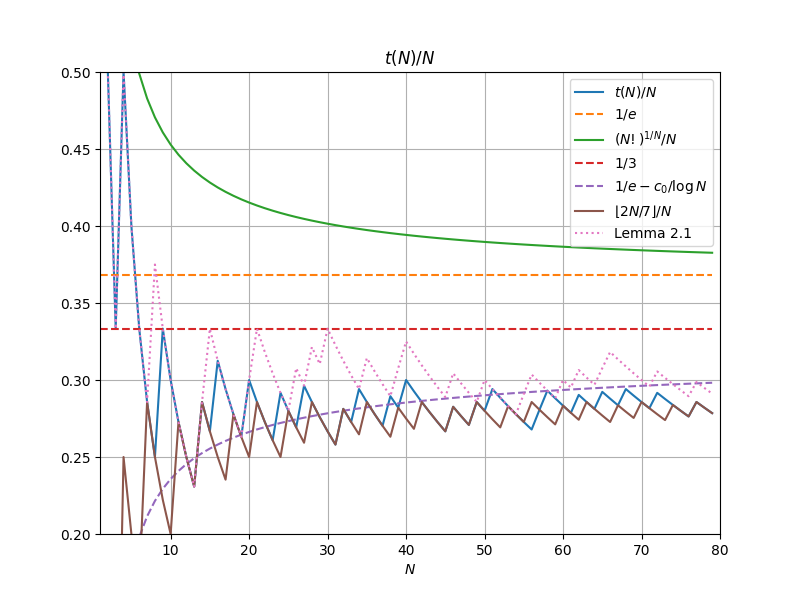
\includegraphics[width=0.8\textwidth]{plot.png}
\caption{The function $t(N)/N$ (blue) for $N \leq 79$, using the data from \href{https://oeis.org/A034258}{OEIS A034258}, as well as the trivial upper bound $(N!)^{1/N}/N$ (green), the improved upper bound from \Cref{upper-crit} (pink), which is asymptotic to \eqref{conjecture} (purple), and the comparison function $\lfloor 2N/7 \rfloor/N$ (brown), which conjecturally is a lower bound for $N \neq 56$ \cite{guy}.  \Cref{main} implies that $t(N)/N$ converges asymptotically to $1/e$ (orange), and we furthermore conjecture the more precise asymptotic \eqref{conjecture} (purple), which crosses $1/3$ (red) at around $N \approx 7000$.}\label{fig1}
\end{figure}

\begin{figure}
  \centering
  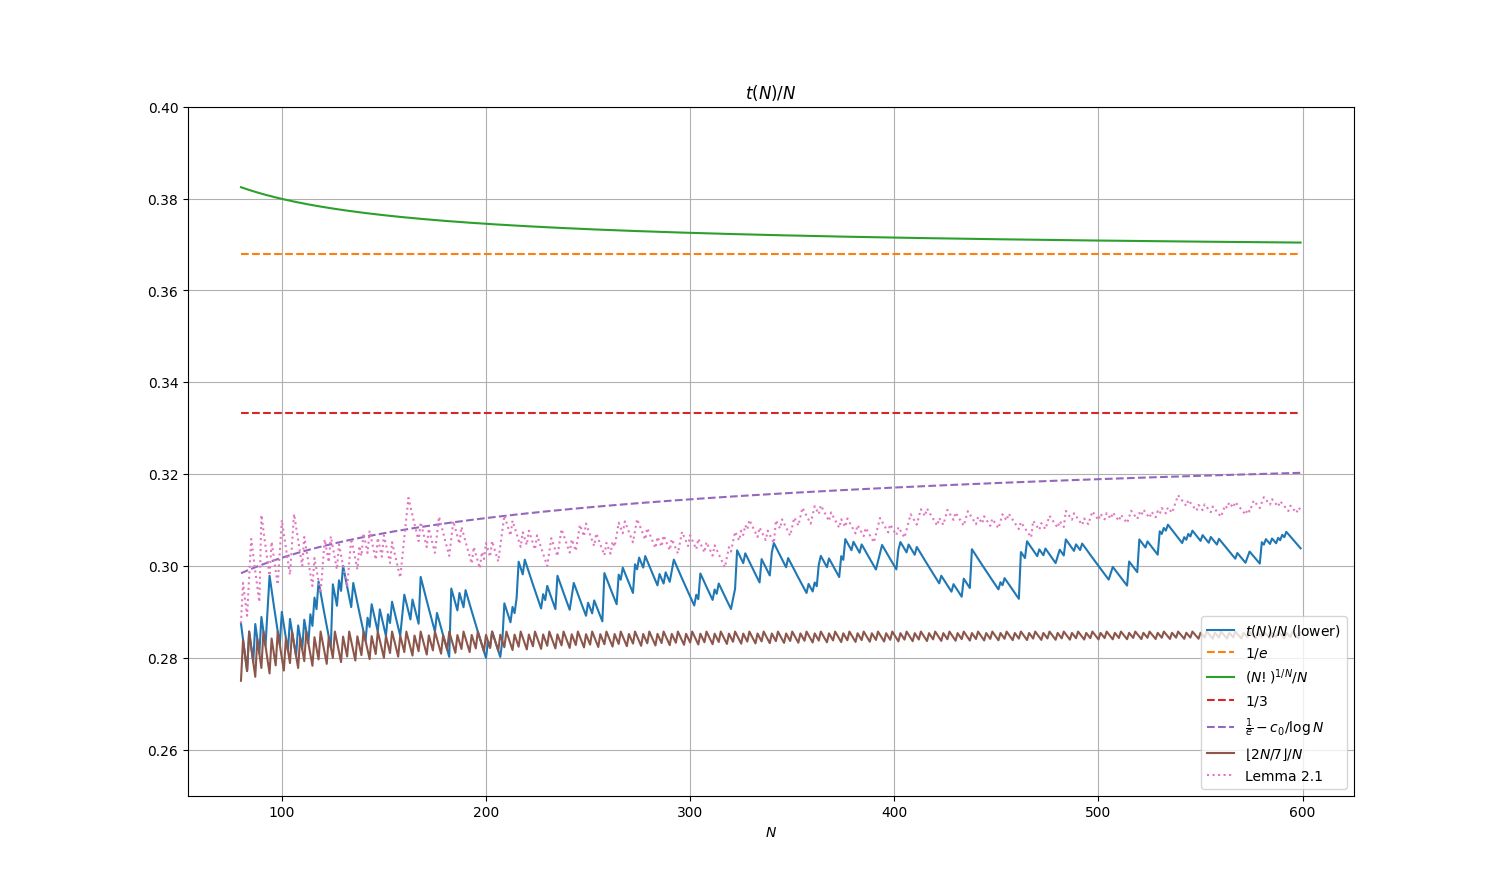
\includegraphics[width=0.8\textwidth]{upperbound.png}
  \caption{A continuation of \Cref{fig1} to the region $80 \leq N \leq 599$.  The data for the function $t(N)/N$ (blue) is only a lower bound, coming from the output of a greedy algorithm provided by Andrew Sutherland.  \Cref{upper-crit} (pink) serves as an upper bound. The three locations $N=182,200,207$ where the conjectured lower bound of $\lfloor 2N/7\rfloor/N$ (brown) is apparently breached can be repaired by using \emph{ad hoc} constructions to improve the lower bound on $t(N)/N$.}\label{fig1-alt}
  \end{figure}

In \cite{guy-selfridge} it is conjectured that $t(N) \geq \lfloor 2N/7\rfloor$ for all $N \neq 56$, that $t(N) \geq N/3$ for\footnote{In \cite{guy-selfridge} it is also asked, ``if [this conjecture is] true, by how much can $\num{300000}$ be reduced?''.} $N \geq \num{300000}$, and that $t(N) < N/e$ for $N \neq 1,2,4$; see \Cref{fig1}.  The proof of the upper bound in \Cref{main} is simple enough that it can be made effective, and the latter conjecture can now be established with some mild computer assistance: see \Cref{tne}.  The other two conjectures can now be attacked numerically.  Andrew Sutherland has kindly provided code\footnote{Links to this code and output may be found at \url{https://terrytao.wordpress.com/2025/03/26}.} to implement a greedy algorithm to factorize $N!$ into products greater than equal to a given threshold $t$, by running through the primes dividing $N!$ in descending order (counting multiplicity) and using, for each such $p$, the smallest $cp$ for which $c$ divides the remaining factors of $N!$.  This provides a lower bound for $t(N)$, which is plotted in \Cref{fig1-alt} for the range $80 \leq N \leq 599$ (and is sharp for $N \leq 79$); in particular, the conjecture $t(N) \geq \lfloor 2N/7 \rfloor$ is verified by this method in this range except for $N = 182, 200, 207$.  Further numerics verify this conjecture for all remaining $N \leq \num{100000}$, while the conjecture $t(N) \geq N/3$ is verified for most $N$ in the range $\num{100000} \leq N \leq \num{5000000}$, including in the range $\num{298344} \leq N \leq \num{300000}$ and for $N$ as large as $\num{490230}$.  Sutherland has also provided some \emph{ad hoc} constructions to resolve the exceptional cases $N = 182, 200, 207$ in the conjecture $t(N) \geq \lfloor 2N/7 \rfloor$.  It seems feasible to completely resolve these conjectures by further numerics, combined with an effective asymptotic analysis to handle extremely large values of $N$.

\subsection{Notation and basic estimates}

We use the usual asymptotic notation $X=O(Y)$, $X \ll Y$, or $Y \gg X$ to denote the bound $|X| \leq CY$ for an absolute constant $C$, and $X=o(Y)$ to denote $|X| \leq c(N) Y$ where $c(N)$ goes to zero as $N \to \infty$. We also write $X \asymp Y$ if $X \ll Y \ll X$.

All sums over $p$ are understood to be over primes.
For any prime $p$ and natural number $n$, we use $\nu_p(n)$ to denote the number of times $p$ divides $n$.  We recall the Legendre formula
\begin{equation}\label{legendre}
  \nu_p(N!) = \sum_{1 \leq j \leq \log N / \log p} \left\lfloor \frac{N}{p^j} \right\rfloor = \frac{N-s_p(N)}{p-1},
\end{equation}
where $s_p(N)$ is the sum of the digits of $N$ in the base $p$ expansion.

We use $\pi(x)$ to denote the number of primes less than or equal to $x$.  We recall the effective prime number theorem from \cite[Corollary 5.2]{dusart}, which asserts that
\begin{equation}\label{pi-lower}
  \pi(x) \geq \frac{x}{\log x} + \frac{x}{\log^2 x}
\end{equation}
for $x \geq 599$ and
\begin{equation}\label{pi-upper}
  \pi(x) \leq \frac{x}{\log x} + \frac{1.2762 x}{\log^2 x}
\end{equation}
for $x >1$.  We also observe from the prime number theorem with classical error term, together with the mean value theorem, that
\begin{equation}\label{pixy}
  \pi(x+y) - \pi(x) = \int_x^{x+y} \frac{dt}{t} + O\left( \frac{x}{\log^{10} x} \right) = \frac{y}{\log x} + O\left( \frac{y^2}{x \log x} \right) + O\left( \frac{x}{\log^{10} x} \right)
  \end{equation}
(say) whenever $2 \leq y \leq x$.

We recall the Stirling approximation in the form of \cite{robbins},
\begin{equation}\label{stirling}
  N \log N - N + \log \sqrt{2\pi N} + \frac{1}{12N+1} \leq \log N! \leq N \log N - N + \log \sqrt{2\pi N} + \frac{1}{12N},
\end{equation}
valid for all natural numbers $N$.  Finally, we recall the standard asymptotic
\begin{equation}\label{harm}
  \sum_{n \leq x} \frac{1}{n} = \log x + \gamma + O\left(\frac{1}{x}\right)
  \end{equation}
for the harmonic series for $x \geq 1$, where $\gamma$ is the Euler--Mascheroni constant.


\section{Proof of upper bound}

We now prove the upper bound in \Cref{main}.  We have a simple criterion to establish such an upper bound:

\begin{lemma}[Upper bound criterion]\label{upper-crit}  Suppose that $1 \leq t \leq N$ are such that
\begin{equation}\label{contra}
   \sum_{p > \frac{t}{\lfloor\sqrt{t}\rfloor}} \left\lfloor \frac{N}{p} \right\rfloor \log \left( \frac{p}{t} \left\lceil \frac{t}{p} \right\rceil \right) > \log N! - N \log t
\end{equation}
Then $t(N) < t$.
\end{lemma}

By optimizing in $t$, this lemma provides an upper bound for $t(N)$ for small and medium values of $N$: see \Cref{fig1} and \Cref{fig1-alt}.

\begin{proof} Suppose for contradiction that $t(N) \geq t$, then we can find $a_1,\dots,a_N \geq t$ such that $N! = a_1 \dots a_N$.  Taking logarithms and rearranging, we conclude that
\begin{equation}\label{ai}
   \sum_{i=1}^N (\log a_i - \log t) = \log N! - N \log t.
\end{equation}
Let $f_t(p) \coloneqq \log (\frac{p}{t} \lceil \frac{t}{p} \rceil)$.  We claim that for any $i$, we have
\begin{equation}\label{ai2}
  \log a_i - \log t \geq f_t(p_{i,1}) + \dots + f_t(p_{i,k})
\end{equation}
where $p_{i,1},\dots,p_{i,k}$ are the primes greater than $\frac{t}{\sqrt{t}+1}$ that divide $a_i$ (counting multiplicity).  For $k=0$ this is clear since $a_i \geq t$.  For $k=1$, we can write $a_i = d_i p_{i,1}$ where $p_{i,1} > \frac{t}{\sqrt{t}+1}$ and $d_i \geq \lceil \frac{t}{p_{i,1}} \rceil$, so that
$$ \log a_i - \log t = \log \left(\frac{p_{i,1}}{t}d_i \right) \geq f_t(p_{i,1})$$
again giving \eqref{ai2}.  For $k \geq 2$, we have $a_i \geq p_{i,1} \dots p_{i,k}$, hence
\begin{align*}
  \log a_i - \log t - \sum_{j=1}^k f_t(p_{i,j}) &\geq \sum_{j=1}^k (\log p_{i,j} - f_t(p_{i,j})) - \log t \\
  &= \sum_{j=1}^k \left(\log t - \log \left \lceil \frac{t}{p_{i,j}} \right\rceil \right) - \log t \\
  &\geq \sum_{j=1}^k \left(\log t - \log \sqrt{t} \right) - \log t \\
  &\geq 0
\end{align*}
which again gives \eqref{ai2}.  By \eqref{legendre}, each prime $p \geq \frac{t}{\sqrt{t}+1}$ appears at least $\lfloor \frac{N}{p}\rfloor$ times in the prime factorization of $a_1 \dots a_N$, thus by \eqref{ai}, \eqref{ai2} we have
$$ \sum_{p \geq \frac{t}{\sqrt{t}+1}} \left\lfloor \frac{N}{p} \right\rfloor f_t(p) \leq \log N! - N \log t,$$
contradicting \eqref{contra}.
\end{proof}

To prove the upper bound, it suffices to show that for any constant $c > c_0$, the criterion \eqref{contra} is satisfied with $t = N/e - cN/\log N$ for $N$ sufficiently large.  By \eqref{stirling}, the right-hand side of \eqref{contra} can be computed to be
$$ \log N! - N \log t = (ec+o(1)) \frac{N}{\log N}.$$
For a fixed $\eps>0$, the left-hand side can be lower bounded for $N$ sufficiently large by
$$
\sum_{\eps N \leq p \leq N} \left\lfloor \frac{N}{p} \right\rfloor \log \left( \frac{p}{t} \left\lceil \frac{t}{p} \right\rceil \right).$$
The summand is piecewise monotone and bounded, with the bounds and the number of pieces uniformly controlled in $N$ for fixed $\eps$ (cf. \Cref{fig-mean}).  A routine application of the prime number theorem \eqref{pi-upper}, \eqref{pi-lower} and summation by parts then computes this sum to be
$$
\frac{1}{\log N} \int_{\eps N}^N \left\lfloor \frac{N}{x} \right\rfloor \log \left( \frac{x}{t} \left\lceil \frac{t}{x} \right\rceil \right)\ dx + o\left(\frac{N}{\log N} \right)$$
or after a change of variables and noting that $t/N = 1/e + o(1)$,
$$
\frac{N}{\log N} \left( \int_{\eps}^1 \left\lfloor \frac{1}{x} \right\rfloor \log \left( ex \left\lceil \frac{1}{ex} \right\rceil \right)\ dx + o(1) \right).
$$
Since $\lceil \frac{1}{ex} \rceil  = \frac{1}{ex} + O(1)$, the integrand is uniformly bounded for $0 < x \leq 1$, and one can write this as
$$
\frac{N}{\log N} (ec_0 + O(\eps) + o(1))
$$
by definition of $c_0$.  For $\eps$ sufficiently small, and then $N$ sufficiently large, we obtain the required conclusion \eqref{contra}.  This completes the proof of the upper bound in \Cref{main}.

A modification of this argument, that is effective for medium values of $N$, resolves the following conjecture of Guy and Selfridge \cite{guy-selfridge}:

\begin{proposition}\label{tne} One has $t(N)/N < 1/e$ for $N \neq 1,2,4$.
\end{proposition}

\begin{proof}  Suppose for contradiction that $t(N)/N \geq 1/e$ for some $N \neq 1,2,4$.
From the data in \href{https://oeis.org/A034258}{OEIS A034258} we may assume that $N \geq 80$ (see \Cref{fig1}).  Applying \Cref{upper-crit}, \eqref{stirling}, it suffices to show that
\begin{equation}\label{test-ineq}
   \sum_{p \geq \frac{N/e}{\lfloor\sqrt{N/e}\rfloor}} \left\lfloor \frac{N}{p} \right\rfloor f_{N/e}(p) > \frac{1}{2} \log(2\pi N) + \frac{1}{12N}
\end{equation}
where $f_{N/e}(p) = \log(\frac{ep}{N} \lceil \frac{N}{ep} \rceil)$ is as in the proof of the proposition.  This is straightforward to verify numerically\footnote{One can also proceed by optimizing \Cref{upper-crit} in $t$; see \Cref{fig1-alt}.} for $80 \leq N < 599$; see \Cref{fig2}.  Hence we may assume $N \geq 599$, where the prime number theorem \eqref{pi-lower} becomes available.

\begin{figure}
  \centering
  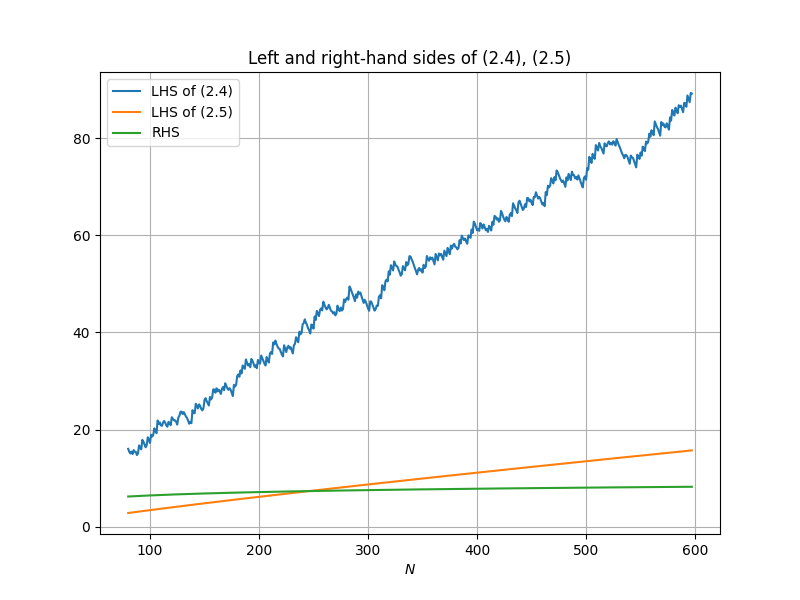
\includegraphics[width=0.8\textwidth]{lhs_rhs.png}
  \caption{A plot of the left and right-hand sides of \eqref{test-ineq}, \eqref{test-2} for $80 \leq N < 599$.  For $N \geq 599$, the effective prime number theorem from \eqref{pi-upper}, \eqref{pi-lower} rigorously establishes the left-hand side of \eqref{test-2} as a lower bound for the left-hand side of \eqref{test-ineq}.}\label{fig2}
\end{figure}

As suggested by \Cref{fig2} (or by noting that the left-hand side is $\asymp N/\log N$, while the right-hand side is $\asymp \log N$), there is significant room to spare here, and we can use somewhat lossy arguments.
For $N/\sqrt{2e} < p \leq N$ one can obtain the lower bound $\lfloor \frac{N}{p} \rfloor f_{N/e}(p) \geq \log (e/2)$ (see \Cref{fig-mean}), and (since $\frac{N/e}{\sqrt{N/e}+1} \geq N/2e$ in the regime $N \geq 599$), so we may crudely bound the left-hand side of \eqref{test-ineq} from below by
$$ \left(\pi(N) - \pi(N/\sqrt{2e})\right) \log(e/2).$$
Applying \eqref{pi-lower}, \eqref{pi-upper}, we reduce to showing that
\begin{equation}\label{test-2}
\begin{split}
  &  \left(\frac{N}{\log N} \left(1 +\frac{1}{\log N}\right)
- \frac{N/\sqrt{2e}}{\log(N/\sqrt{2e})} \left(1 +\frac{1.2762}{\log(N/\sqrt{2e})}\right)\right) \log (e/2) \\
&\quad > \frac{1}{2} \log(2\pi N) + \frac{1}{12N}
\end{split}
\end{equation}
for $N \geq 599$. This can be numerically verified for $N=599$ (see Figure \ref{fig2}), so by the fundamental theorem of calculus it suffices to show that the derivative of the left-hand side is at least that of the right hand side for (real) $N \geq 599$.  Computing this derivative, dividing by $\log(e/2)$, and discarding some terms with a favorable sign, we reduce to showing that
$$ \frac{1}{\log N} - \frac{2}{\log^3 N} - \frac{1}{\sqrt{2e} \log(N/\sqrt{2e})} - \frac{0.2762}{\sqrt{2e} \log^2(N/\sqrt{2e})}  \geq \frac{1}{2\log(e/2) N}$$
for $N \geq 599$.  But in this range we have the crude lower bounds $\log N \geq \log(N/\sqrt{2e})\geq 5$, $\sqrt{2e} \log(N/\sqrt{2e}) \geq 2 \log N$, and $2 \log(e/2) N \geq 50 \log N$, and the claim then follows (with room to spare) by estimating all terms here by constant multiples of $\frac{1}{\log N}$.
\end{proof}

\section{Proof of lower bound}

We now establish the lower bound.  We need to find a sequence of exactly $N$ numbers $a_1,\dots,a_N$, which multiply to exactly $N!$ (or equivalently by the fundamental theorem of arithmetic, that $\sum_{i=1}^N \nu_p(a_i)=  \nu_p(N!)$ for all $p$), and such that $a_i \geq N/e - O(N/\log N)$ for all $i$.  These are somewhat rigid constraints.  We therefore perform a preliminary reduction\footnote{The logical ordering of the arguments in this section, in which we pass from the $a_i$ to the $b_i$ to the $c_i$, are the reverse of the outline of the construction given in the introduction, which first described the $c_i$ and then constructed the $b_i$ and finally the $a_i$.} to relax the constraints by allowing some exceptional elements of the sequence to be small, to allow the number $N'$ of elements of the sequence to deviate slightly from $N$, and by permitting the sum $\sum_{i=1}^N \nu_p(a_i)$ to deviate slightly from $\nu_p(N!)$ for odd $p$ (and to abandon direct control of this sum for $p=2$).  More precisely, we will use the following lower bound criterion.


\begin{proposition}[Lower bound criterion]\label{lower bound} Let $\delta>0$ and $N \geq e^{1+\delta}$. Let $b_1,\dots,b_{N'}$ be a sequence of natural numbers, and define the following quantities:
  \begin{itemize}
    \item[(i)] $D_1$ is the number of $i=1,\dots,N'$ such that $b_i < N / e^{1+\delta}$.
    \item[(ii)] $D_2 \coloneqq \sum_{i=1}^{N'} (\log b_i - \log (N/e^{1+\delta}))_+$.
    \item[(iii)] $D_3 \coloneqq \sum_{p>2} (\sum_{i=1}^{N'} \nu_p(b_i) - \nu_p(N!))_+$.
    \item[(iv)] $D_4 \coloneqq \sum_{p>2} (\nu_p(N!) - \sum_{i=1}^{N'} \nu_p(b_i))_+ \log p$.
  \end{itemize}
Here $x_+ \coloneqq \max(x,0)$.
If one has the inequality
\begin{equation}\label{d24}
   D_2 + D_4 + (D_1 + D_3) \log 2 + |N'-N| \log N \leq \delta N,
\end{equation}
then
$$ t(N) \geq \frac{N}{e^{1+\delta}}.$$
\end{proposition}

\begin{proof}
  We first observe that we can perform a number of ``cleaning'' moves to improve the properties of the $b_i$, as follows.

  \begin{itemize}
  \item (Adding dummy elements) By adding $(N-N')_+$ dummy elements $b_i=1$, which increments $D_1$ by at most $(N-N')_+$ without affecting $D_2,D_3,D_4$ (and thus preserving \eqref{d24}), we may assume without loss of generality that $N' \leq N$.
  \item (Removing excess primes) If $\sum_{i=1}^{N} \nu_p(b_i) > \nu_p(N!)$ for some $p>2$, one may divide one of the $b_i$ by $p$, thus reducing $D_3$ by one, and incrementing $D_1$ by at most one, leaving $D_3,D_4,N'$ unchanged (thus preserving \eqref{d24}).  Iterating this, we may thus assume that $D_3=0$, thus
  \begin{equation}\label{nupi}
    \sum_{i=1}^{N} \nu_p(b_i) \leq \nu_p(N!)
   \end{equation}
     for all $p>2$.
  \item (Inflating small factors) If $1 \leq i \leq N$ and $k \geq 1$ are such that $(k-1) \log 2 < \log (N/e^{1+\delta})- \log b_i \leq k \log 2$, then if one replaces $b_i$ by $2^k b_i$, then this decreases $D_1$ by one, while increasing $D_2$ by at most $\log 2$, with $D_3,D_4,N'$ (and \eqref{nupi}) unaffected, thus preserving \eqref{d24}.  Iterating this procedure, we may thus assume that $D_1=0$, thus $b_i \geq N/e^{1+\delta}$ for all $i=1,\dots,N$.
  \end{itemize}

Since $D_1=0$, we have
  $$ \sum_{i=1}^{N'} (\log b_i - \log (N/e^{1+\delta})) = D_2$$
  or equivalently
  $$ \sum_{i=1}^{N'} \log b_i = N' \log N - N' - \delta N' + D_2.$$
  We can upper bound this by
  $$ \sum_{i=1}^{N'} \log b_i \leq N \log N - N - \delta N + |N'-N| \log N + D_2.$$
  By the fundamental theorem of arithmetic, we can expand the left-hand side as
  $$ \sum_p \sum_{i=1}^{N'} \nu_p(b_i) \log p.$$
  Meanwhile, from \eqref{nupi} we have
  $$\sum_{p>2} \left(\nu_p(N!) - \sum_{i=1}^{N'} \nu_p(b_i)\right) \log p = D_4$$
  and thus
  $$ \sum_{i=1}^{N'} \nu_2(b_i) \log p
  \leq N \log N - N - \delta N - \sum_{p>2} \nu_p(N!) \log p + |N'-N|  \log N + D_2 + D_4.$$
  From \eqref{stirling} one has
  $$ \sum_p \nu_p(N!) \log p = \log N! \geq N \log N - N$$
  and hence
  $$ \sum_{i=1}^{N'} \nu_2(b_i) \log 2 \leq \nu_2(N!) \log 2 - \delta N + |N'-N| \log N + D_2 + D_4.$$
  so we conclude from \eqref{delta-def} that
  $$ \sum_{i=1}^{N'} \nu_2(b_i) \leq \nu_2(N!).$$
  From this, \eqref{nupi}, and the fundamental theorem of arithmetic, we conclude that $b_1 \dots b_{N'}$ divides $N!$.  If we multiply (say) $b_1$ by the remaining factor of $N! / b_1 \dots b_{N'}$, and concatenate $b_{N},\dots,b_{N'}$ into a single number $b_{N} \dots b_{N'}$, we obtain a new sequence $a_1,\dots,a_N$ with $a_1 \dots a_N = N!$ and $a_i \geq N/e^{1+\delta}$ for all $i$, so that $t(N) \geq N / e^{1+\delta}$, giving the required lower bound.
\end{proof}

In view of \Cref{lower bound}, the lower bound in \Cref{main} will be immediate from the following proposition.

\begin{proposition}[Key proposition]\label{key-prop}  Let $C_0 > 1$, and let $N$ be sufficiently large depending on $C_0$.  Set
  \begin{equation}\label{delta-def}
    \delta \coloneqq \frac{C_0}{\log N}.
  \end{equation}
Then there exists $N' = N + O(N/\log^2 N)$ and natural numbers $b_1,\dots,b_{N'}$ obeying the following axioms.
\begin{itemize}
\item[(i)] One has $b_i  \geq N/e^{1+\delta}$ for all but $O(N/\log N)$ of the $i=1,\dots,N'$.
\item[(ii)] One has
$\sum_{i=1}^{N'} (\log b_i - \log (N/e^{1+\delta}))_+ \ll \frac{N}{\log N}$.
\item[(iii)] One has
 $\sum_{p>2} (\sum_{i=1}^{N'} \nu_p(b_i) - \nu_p(N!))_+ \ll \frac{N}{\log N}$.
\item[(iv)] One has
 $\sum_{p>2} (\nu_p(N!) - \sum_{i=1}^{N'} \nu_p(b_i))_+ \log p \ll \frac{N}{\log N}$.
\end{itemize}
The implied constants in the asymptotic notation do not depend on $C_0$.
\end{proposition}

Informally, (i) and (ii) assert that the $b_i$ are usually slightly larger than $N/e^{1+\delta}$, while (iii) and (iv) assert that $\sum_{i=1}^{N'} \nu_p(b_i)$ is usually slightly smaller than $\nu_p(N!)$ for odd primes $p$.

It remains to prove \Cref{key-prop}.  We begin by constructing a preliminary sequence
$$c_1,\dots,c_{N'}$$
that obeys most of the axioms (i)-(iv) required for \Cref{key-prop}, except at large primes where there is significant discrepancy between $\sum_i \nu_p(c_i)$ and $\nu_p(N!)$; informally, $c_1 \dots c_{N'}$ contains the ``wrong'' set of large prime factors, but has essentially the ``correct'' set of small prime factors.  We will then modify this sequence $c_i$ by replacing many of large prime factors of $c_i$ with large (and usually nearby) prime factors of $N!$ to obtain the required sequence $b_i$.

We turn to the details.  We introduce the moderately large power of two
\begin{equation}\label{A-def}
   A \coloneqq 2^{\lfloor \log^3 N / \log 2 \rfloor} \asymp \log^3 N,
\end{equation}
and let $I$ denote the set of odd natural numbers in the interval
$$ \left[\frac{N}{e^{1+\delta}}, \frac{N}{e^{1+\delta}} + \frac{N}{A}\right].$$
Clearly $I$ has cardinality $N/2A + O(1)$.  Thus, if we set $N' \coloneqq 2A|I|$, then we have
\begin{equation}\label{N'-card}
  N' = N + O(A) = N + O\left( \frac{N}{\log^2 N}\right).
\end{equation}
We now set $c_1,\dots,c_{N'}$ to be the elements of $I$, each repeated with multiplicity $2A$; the ordering of the $c_1,\dots,c_{N'}$ will not be of relevance to us.  Clearly we have $c_i \geq N/e^{1+\delta}$ for all $i$, and
\begin{equation}\label{cii}
   \sum_{i=1}^{N'} (\log c_i - \log (N/e^{1+\delta}))_+ \ll \frac{N}{A} \ll \frac{N}{\log N};
\end{equation}
thus the analogues of axioms (i) and (ii) are satisfied.  Now we study axioms (iii), (iv).  Call a prime $p$ \emph{small} if $p \leq N/A^2$, and \emph{large} if $p > N/A^2$.  For a small odd prime $2 < p \leq N/A^2$, we see from \eqref{legendre} that
$$ \nu_p(N!) = \frac{N}{p-1} + O(\log N).$$
In a similar spirit, the quantity $\sum_{i=1}^{N'} \nu_p(c_i)$ can be computed as
\begin{align*}
  \sum_{i=1}^{N'} \nu_p(c_i) &= 2A \sum_{1 \leq j \leq \log N/\log p} |I \cap p^j \Z| \\
  &= 2A \sum_{1 \leq j \leq \log N/\log p} \left(\frac{N}{2Ap^j} + O(1)\right) \\
  &= \frac{N}{p-1} + O(A \log N)
\end{align*}
and hence we have good agreement between $c_1 \dots c_{N'}$ and $N!$ at small primes:
\begin{equation}\label{nupci}
   \sum_{i=1}^{N'} \nu_p(c_i) = \nu_p(N!) + O(A \log N).
\end{equation}
From this, the triangle inequality, and \eqref{A-def}, we easily obtain the bounds
\begin{equation}\label{ciii}
  \sum_{2 < p \leq N/A^2} \left(\sum_{i=1}^{N'} \nu_p(c_i) - \nu_p(N!)\right)_+ \ll \frac{N}{\log N}
\end{equation}
and
\begin{equation}\label{civ}
  \sum_{2 < p \leq N/A^2} \left(\nu_p(N!) - \sum_{i=1}^{N'} \nu_p(c_i)\right)_+ \log p \ll \frac{N}{\log N}
\end{equation}
(with some powers of $\log N$ to spare).  So we have the analogue of axioms (iii), (iv) for small primes; the main difficulty is with the large primes.

Let us enumerate all the large primes dividing $N!$ (counting multiplicity) in order as $p_1 \leq \dots \leq p_M$; these primes range between $N/A^2$ and $N$, so in particular
\begin{equation}\label{log-p}
  \log p_m = \log N + O(\log \log N)
\end{equation}
for $m=1,\dots,M$.  By \eqref{legendre}, each large prime $p$ divides $N!$ exactly $\lfloor N/p \rfloor$ times, so we have
\begin{align}
  M &= \sum_{N/A^2 < p \leq N} \left \lfloor \frac{N}{p} \right \rfloor \nonumber \\
  &= \sum_{k=1}^{A^2} \sum_{N/K < p \leq N/k} 1 \nonumber \\
  &= \sum_{k=1}^{A^2} \left(\frac{N}{k\log N} - \frac{N}{K \log N} + O\left( \frac{N \log k}{\log^2 N} \right)\right)  \nonumber \\
  &= \frac{N}{\log N} (\log A^2 + \gamma - 1 + o(1)) \label{gamma}\\
  &= O\left( \frac{N \log\log N}{\log N} \right)\nonumber
\end{align}
thanks to \eqref{pi-upper}, \eqref{pi-lower}, \eqref{harm}.

We similarly enumerate the large primes dividing $c_1 \dots c_{N'}$ (counting multiplicity) as $p'_1 \leq \dots \leq p'_{M'}$; these primes range between $N/A^2$ and $N/e$, so in particular
\begin{equation}\label{log-pp}
  \log p'_{m'} = \log N + O(\log \log N)
\end{equation}
for $m'=1,\dots,M'$.  We can compute $M'$ indirectly as follows.  From the fundamental theorem of arithmetic and \eqref{nupci}, \eqref{log-pp}, \eqref{log-p} we have
\begin{align*}
\sum_{i=1}^{N'} \log c_i &= \sum_{p>2} \sum_{i=1}^{N'} \nu_p(c_i) \log p \\
&= \sum_{2 < p \leq N/A^2}  \sum_{i=1}^{N'} \nu_p(c_i) \log p + \log p'_1 + \dots + \log p'_{M'} \\
&= \sum_{2 < p \leq N/A^2}  \nu_p(N!) \log p + O\left( A \log N \frac{N}{A^2} \right) + M' (\log N + O(\log \log N)) \\
&= \log N! - \nu_2(N!) \log 2 - \log p_1 - \dots - \log p_M \\
&\quad + O\left( \frac{N\log N }{A} \right) + M' (\log N + O(\log\log N)).
\end{align*}
Applying \eqref{stirling}, \eqref{legendre} we conclude that
\begin{align*}
  \sum_{i=1}^{N'} \log c_i &= N \log N - N - N \log 2 - M (\log N + O(\log\log N)) \\
&\quad  + O\left( \frac{N\log N }{A} \right) + M' (\log N + O(\log\log N)) \\
&= N \log N - N - N \log 2 + (M'-M) (\log N + O(\log\log N)) \\
&\quad + O\left( \frac{N\log N }{A} \right) + O\left( \frac{N(\log\log N)^2}{\log N} \right) \\
&= N \log N - N - N \log 2 + (1+o(1)) (M'-M) \log N  + o(N).
\end{align*}
On the other hand, from the construction of $c_i$ we have $\log c_i = \log N/e^{1+\delta} + O(1/A) = \log N - 1 + o(1)$ for all $i$, hence
\begin{align*}
  \sum_{i=1}^{N'} \log c_i &= N' (\log N - 1 - o(1)) \\
  &= N \log N - N + o(N)
\end{align*}
thanks to \eqref{N'-card}. Equating the two estimates, we conclude that
\begin{equation}\label{Mdiff}
  M'-M = (\log 2 + o(1)) \frac{N}{\log N}.
\end{equation}
In particular, $M' \geq M$.  That is to say, $c_1 \dots c_{N'}$ contains more\footnote{This is to be expected, since $c_1 \dots c_{N'}$ contains no factors of $2$, whereas $N!$ contains about $N$ of them.} large primes in its factorization than $N!$.

Now suppose that we can assign a large prime $p'_{\sigma(m)}$ in the factorization of $c_1 \dots c_{N'}$ to each large prime $p_m$ in the factorization of $N!$ for $m=1,\dots,M$, obeying the following axioms:
\begin{itemize}
\item[(a)]  The map $\sigma \colon\{1,\dots,M\} \to\{1,\dots,M'\}$ is injective.
\item[(b)]  One has $p_m \geq p'_{\sigma(m)}$ for all but at most $O(N/\log N)$ choices of $m = 1,\dots,M$.
\item[(c)] One has $\sum_{m=1}^M (\log p_m - \log p'_{\sigma(m)})_+ \ll N/\log N$.
\end{itemize}
(Informally, (b) and (c) assert that $p'_{\sigma(m)}$ is usually a little bit smaller than $p_m$.)  Then we can modify the sequence $c_1,\dots,c_{N'}$ to a new sequence $b_1,\dots,b_{N'}$ by, for each $m=1,\dots,M$, replacing the occurrence of $p'_{\sigma(m)}$ in the appropriate $c_i$ with $p_m$ instead.  By axiom (b), we will have $b_i \geq c_i$ with at most $O(N/\log N)$ exceptions, giving axiom (i).  From the triangle inequality we have
$$ \sum_{i=1}^{N'} (\log b_i - \log (N/e^{1+\delta}))_+ \leq \sum_{i=1}^{N'} (\log c_i - \log (N/e^{1+\delta}))_+ + \sum_{m=1}^M (\log p_m - \log p'_{\sigma(m)})_+$$
and so axiom (ii) follows from axiom (c) and \eqref{cii}.  Every large prime $p_1,\dots,p_M$ in the factorization of $N!$ is used in $b_1 \dots b_{N'}$, so the contribution of large primes to axiom (iv) is trivial, and the contribution of small primes is acceptable from \eqref{civ}.  Finally, by construction there are only $M'-M = O(N/\log N)$ large primes in $b_1 \dots b_{N'}$ that are in excess of the large primes $p_1,\dots,p_M$ needed to factorize $N!$, so from this and \eqref{ciii} we recover axiom (iii).  Thus we will be able to establish \Cref{key-prop} as soon as we can find an assignment $m \mapsto \sigma(m)$ obeying the axioms (a), (b), (c).

The large primes $p_1,\dots,p_M$ and $p'_1,\dots,p'_{M'}$ all lie in the interval $J \coloneqq (N/A^2, N]$.  We select a large natural number constant $K_0$ (and assume $N$ sufficiently large depending on $K_0$), and break the interval $J$ up into the dyadic intervals $J_k \coloneqq (N/2^k, N/2^{k-1}]$ for $2^{K_0} < 2^k \leq A^2$ (so in particular $k=O(\log\log N)$), together with the remaining interval $J_* \coloneqq (N/2^{K_0},N]$.  In order to achieve the axioms (b), (c), we will try to match primes $p_m$ in a dyadic interval $J_k$ to primes $p'_{j_m}$ in the same dyadic interval $J_k$, only resorting to the remaining interval $J_*$ when an appropriate match within the same interval is not available.

We first understand the distribution of the primes $p_m$ inside a given dyadic interval $J_k$.  It will be convenient to introduce the error tolerance
\begin{equation}\label{eps-def}
   \eps_k \coloneqq \frac{(\log\log N)^2}{\log N} + \frac{1}{2^k}.
\end{equation}
For future reference we observe the bound
\begin{equation}\label{eps-sum}
\sum_{2^{K_0} < 2^k \leq A^2} \eps_k \ll 2^{-K_0}.
\end{equation}


By \eqref{legendre}, each prime $p$ in $J_k$ appears $\lfloor N/p\rfloor$ times, so the number $M_k$ of times $p_m$ lies in this interval is given by
\begin{align*}
  M_k &= \sum_{N/2^k < p \leq N/2^{k-1}} \left\lfloor \frac{N}{p} \right\rfloor \\
  &= \sum_{N/2^k < p \leq N/2^{k-1}} \frac{N}{p} + O\left( \frac{N}{2^k \log N} \right) \\
  &= N(\log\log(N/2^{k-1}) - \log\log(N/2^k)) + O\left( \frac{N}{2^k \log N}\right)\\
  &= \log 2 \frac{N}{\log N} + O\left( \frac{\eps_k N}{\log N} \right)
\end{align*}
using Mertens' theorem with the classical error term coming from the prime number theorem (or by \eqref{pi-upper}, \eqref{pi-lower}, and summation by parts), followed by the mean value theorem and \eqref{eps-def}.

The number $M_*$ of primes $p_m$ in the remaining interval $J_*$ can then be computed using \eqref{gamma}, \eqref{eps-sum} to be
\begin{equation}\label{ms}
 M_* = M - \sum_{2^{K_0} < 2^k \leq A^2} M_k = \frac{N}{\log N} (\log 2^{K_0} + \gamma - 1 + O(2^{-K_0}) ).
\end{equation}
A similar calculation shows that for any $N/2^k \leq R \leq N/2^{k-1}$, the number of $p_m$ in $(N/2^k, R]$ is equal to
$N(\log\log R - \log\log(N/2^k)) + O( \eps_k \frac{N}{\log N} )$, which simplifies by the mean value theorem and \eqref{eps-def} to
$N\frac{\log \frac{2^k R}{N}}{\log N} + O( \eps_k \frac{N}{\log N} )$
.  Thus, if we enumerate the $M_k$ primes from $p_1,\dots,p_M$ that lie in $J_k$ as $p_{k,1} \leq \dots \leq p_{k,M_k}$, one has
$$ m = N\frac{\log \frac{2^k p_{k,m}}{N}}{\log N} + O\left( \eps_k \frac{N}{\log N} \right)$$
for all $m=1,\dots,M_k$, and hence we have an approximate formula for $p_{k,m}$:
$$ p_{k,m} = (1 + O(\eps_k)) \exp\left( \frac{m \log N}{N} \right) \frac{N}{2^k}.$$

Now we understand the distribution of primes $p'_{m'}$ inside the same interval $J_k$.  The $c_i$ that generate a large prime $p'_{m'}$ in this interval take the form $c_i = d_i p_i$, where $2^{k-1}/e^{1+\delta} - O(2^k/A) \leq d_i \leq 2^k/e^{1+\delta} + O(2^k/A)$ is an odd number and $p_i$ is a large prime in the interval
$$ (N/2^k, N/2^{k-1}] \cap \left[\frac{N}{e^{1+\delta} d_i}, \frac{N}{e^{1+\delta} d_i} + \frac{N}{A d_i}\right].$$
Furthermore, each such pair $d_i,p_i$ contributes $2A$ such large primes to the this interval.  For a fixed odd choice $d$ of $d_i$ in ths indicated range, the number of large primes $p_i$ appearing in this fashion can be computed by the prime number theorem with classical error term \eqref{pixy} to be $\frac{N}{A d \log N} + O( \frac{N \log\log N}{Ad \log^2 N})$ except in the endpoint cases $d = 2^k/e^{1+\delta} + O(2^k/A)$, $d = 2^{k-1}/e^{1+\delta} + O(2^k/A)$, in which case the Brun--Titchmarsh theorem (or \eqref{pixy} again) gives the upper bound $O(\frac{N}{A 2^k \log N})$.  The total number $M'_k$ of large primes $p'_m$ in this interval coming from the factorization of $c_1 \dots c_{N'}$ can then be computed to be
\begin{align*}
  M'_k &= 2A \left(\sum_{2^{k-1} < d \leq 2^k,\ \mathrm{odd}} \left(\frac{N}{A d \log N} + O\left( \frac{N \log\log N}{Ad \log^2 N}\right)\right) + O\left( \frac{2^k}{A} \frac{N}{A 2^k \log N} \right)\right) \\
&= \log 2 \frac{N}{\log N} + O\left( \eps_k \frac{N}{\log N} \right) \\
&= M_k + O\left( \eps_k \frac{N}{\log N} \right).
\end{align*}
The number $M'_*$ of primes $p'_m$ in the remaining interval $J_*$ can then be computed using \eqref{ms}, \eqref{Mdiff}, \eqref{eps-sum} as
\begin{equation}\label{msp}
  M'_* = M' - \sum_{2^{K_0} < 2^k \leq A^2} M'_k = M_* + \frac{N}{\log N} (\log 2 + O(2^{-K_0}) ).
 \end{equation}
 A similar calculation shows that for any $N/2^k \leq R \leq N/2^{k-1}$, the number of $p'_m$ in $(N/2^k, R]$ is equal to
 $N\frac{\log \frac{2^k R}{N}}{\log N} + O( \eps_k \frac{N}{\log N} )$, so if we enumerate the $M'_m$ primes in $J_k$ as $p'_{k,1} \leq \dots \leq p'_{k',M_k}$, then as before we have
$$ p'_{k,m} = (1 + O(\eps_k)) \exp\left( \frac{m \log N}{N} \right) \frac{N}{2^k}.$$
In particular, from the mean value theorem we have
$$ p'_{k,m-H_k} \leq p_{k,m} \leq (1 + O(\eps_k)) p'_{k,m-H_k}$$
for some $H_k \asymp \eps_k \frac{N}{\log N}$ and all $H_k < m \leq M_k$.  If we then assign $p'_{k,m-H_k}$ to $p_{k,m}$ for each such $k,m$, then this assignment creates no violations of axioms (a) and (b), while contributing at most
$$ \sum_{2^{K_0} < 2^k \leq A^2} M_k O(\eps_k) \ll \frac{N}{\log N} \sum_{2^{K_0} < 2^k \leq A^2} \eps_k \ll 2^{-K_0} \frac{N}{\log N} $$
to the sum in (c), thanks to \eqref{eps-sum}.  This leaves $H_k$ of the primes $p_{k,m}$ still unassigned for $2^{K_0} < 2^k \leq A^2$.  To each such prime, we assign arbitrarily a prime $p_{m'}$ in $J_*$ from the factorization of $c_1 \dots c_{N'}$; since by \eqref{eps-sum}
$$ \sum_{2^{K_0} < 2^k \leq A^2} H_k \ll \sum_{2^{K_0} < 2^k \leq A^2} \eps_k \frac{N}{\log N} \ll 2^{-K_0} \frac{N}{\log N}$$
is much smaller than $M'_* \asymp \frac{N}{\log N}$, there is no difficulty making this assignment injective, so that axiom (a) remains preserved.  Each assignment creates a violation of (b), but the total number of such violations is $\ll 2^{-K_0} \frac{N}{\log N}$, which is acceptable; and axiom (c) remains unaffected.

Finally, we need to assign an unused prime $p_{m'}$ in the factorization of $c_1 \dots c_{N'}$ to each prime $p_m$ in $J_*$ in the factorization of $N!$.  The number of primes we have to assign is $M_*$.  By \eqref{msp} we see that, even after removing the $\sum_{2^{K_0} < 2^k \leq A^2} H_k = O( 2^{-K_0} \frac{N}{\log N})$ primes $p_{m'}$ in $J_*$ that were previously assigned, there are still $M_* + \frac{N}{\log N} (\log 2 + O(2^{-K_0}) )$ primes $p_{m'}$ available; in particular, if $K_0$ is large enough, there are at least $M_*$ such primes.  We then make an arbitrary injective assignment of such primes to each $p$ in $J_*$ in the factorization of $N!$, preserving axiom (a); this can create up to $M_* \asymp K_0 N / \log N$ violations of axiom (b), but this is acceptable by taking $K_0$ to be a large constant.  Similarly, the net contribution to (c) is at most $M_* \log 2^{K_0} = O(K_0^2 N / \log N)$, which is also acceptable.  This completes the construction of the desired assignment $m \mapsto \sigma(m)$ obeying the required axioms (a), (b), (c), and the proof of the lower bound in \Cref{main} is now complete.

 \subsection{Acknowledgements}

The author is supported by NSF grant DMS-2347850.  We thank Thomas Bloom for the web site \url{https://www.erdosproblems.com}, where the author learned of this problem, as well as Bryna Kra and Ivan Pan for  corrections. We are particularly indebted to Andrew Sutherland for supplying numerics and code to lower bound $t(N)$ for various medium-sized values of $N$.

\begin{thebibliography}{10}

\bibitem{algr77}
K. Alladi, C. Grinstead, \emph{On the decomposition of $n!$ into prime powers}, J. Number Theory \textbf{9} (1977) 452--458.

\bibitem{bincover}
S. F. Assmann, D. S. Johnson, D. J. Kleitman, J. Y.-T. Leung, \emph{On a dual version of the one-dimensional bin packing problem}, J. Algorithms \textbf{5} (1984) 502--525.

\bibitem{dusart}
P. Dusart, \emph{Explicit estimates of some functions over primes}, Ramanujan J. \textbf{45} (2018) 227--251.

\bibitem{erdos-71}
P. Erd\H{o}s, \emph{Some problems in number theory}, in Computers in Number Theory, Academic Press, London New York, 1971, pp. 405--414.

\bibitem{erdos-96}
P. Erd\H{o}s, \emph{Some problems I presented or planned to present in my short talk}, Analytic number theory, Vol. 1 (Allerton Park, IL, 1995) (1996), 333--335.

\bibitem{erdos-graham}
P. Erd\H{o}s, R. Graham, \emph{Old and new problems and results in combinatorial number theory}, Monographies de L'Enseignement Mathematique 1980.

\bibitem{guy}
R. K. Guy, \emph{Unsolved Problems in Number Theory}, 3rd Edition, Springer, 2004.

\bibitem{guy-selfridge}
R. K. Guy, J. L. Selfridge, \emph{Factoring factorial $n$}, Amer. Math. Monthly \textbf{105} (1998) 766--767.

\bibitem{robbins}
H. Robbins, \emph{A Remark on Stirling's Formula}, Amer. Math. Monthly \textbf{62} (1955) 26--29.

\end{thebibliography}


\end{document}
